%%%%%%%% ICML 2023 EXAMPLE LATEX SUBMISSION FILE %%%%%%%%%%%%%%%%%

\documentclass{article}

% Recommended, but optional, packages for figures and better typesetting:
\usepackage{microtype}
\usepackage{graphicx}
\usepackage{subfigure}
\usepackage{booktabs} % for professional tables

\usepackage{tikz}
% Corporate Design of the University of Tübingen
% Primary Colors
\definecolor{TUred}{RGB}{165,30,55}
\definecolor{TUgold}{RGB}{180,160,105}
\definecolor{TUdark}{RGB}{50,65,75}
\definecolor{TUgray}{RGB}{175,179,183}

% Secondary Colors
\definecolor{TUdarkblue}{RGB}{65,90,140}
\definecolor{TUblue}{RGB}{0,105,170}
\definecolor{TUlightblue}{RGB}{80,170,200}
\definecolor{TUlightgreen}{RGB}{130,185,160}
\definecolor{TUgreen}{RGB}{125,165,75}
\definecolor{TUdarkgreen}{RGB}{50,110,30}
\definecolor{TUocre}{RGB}{200,80,60}
\definecolor{TUviolet}{RGB}{175,110,150}
\definecolor{TUmauve}{RGB}{180,160,150}
\definecolor{TUbeige}{RGB}{215,180,105}
\definecolor{TUorange}{RGB}{210,150,0}
\definecolor{TUbrown}{RGB}{145,105,70}

% hyperref makes hyperlinks in the resulting PDF.
% If your build breaks (sometimes temporarily if a hyperlink spans a page)
% please comment out the following usepackage line and replace
% \usepackage{icml2023} with \usepackage[nohyperref]{icml2023} above.
\usepackage{hyperref}


% Attempt to make hyperref and algorithmic work together better:
\newcommand{\theHalgorithm}{\arabic{algorithm}}

\usepackage[accepted]{icml2023}

% For theorems and such
\usepackage{amsmath}
\usepackage{amssymb}
\usepackage{mathtools}
\usepackage{amsthm}

% if you use cleveref..
\usepackage[capitalize,noabbrev]{cleveref}

%%%%%%%%%%%%%%%%%%%%%%%%%%%%%%%%
% THEOREMS
%%%%%%%%%%%%%%%%%%%%%%%%%%%%%%%%
\theoremstyle{plain}
\newtheorem{theorem}{Theorem}[section]
\newtheorem{proposition}[theorem]{Proposition}
\newtheorem{lemma}[theorem]{Lemma}
\newtheorem{corollary}[theorem]{Corollary}
\theoremstyle{definition}
\newtheorem{definition}[theorem]{Definition}
\newtheorem{assumption}[theorem]{Assumption}
\theoremstyle{remark}
\newtheorem{remark}[theorem]{Remark}

% Formular
\usepackage{array,tabularx}
\newenvironment{conditions*}
  {\par\vspace{\abovedisplayskip}\noindent
   \tabularx{\columnwidth}{>{$}l<{$} @{\ : } >{\raggedright\arraybackslash}X}}
  {\endtabularx\par\vspace{\belowdisplayskip}}

% Quelle
\newcommand*{\quelle}{
  \footnotesize Imagesource: Inverted image from\\
}

% Todonotes is useful during development; simply uncomment the next line
%    and comment out the line below the next line to turn off comments
%\usepackage[disable,textsize=tiny]{todonotes}
\usepackage[textsize=tiny]{todonotes}


% The \icmltitle you define below is probably too long as a header.
% Therefore, a short form for the running title is supplied here:
\icmltitlerunning{Project Report Template for Data Literacy 2023/24}

\begin{document}

\twocolumn[
\icmltitle{The Evolution of Design Complexity in LEGO Sets}

% It is OKAY to include author information, even for blind
% submissions: the style file will automatically remove it for you
% unless you've provided the [accepted] option to the icml2023
% package.

% List of affiliations: The first argument should be a (short)
% identifier you will use later to specify author affiliations
% Academic affiliations should list Department, University, City, Region, Country
% Industry affiliations should list Company, City, Region, Country

% You can specify symbols, otherwise they are numbered in order.
% Ideally, you should not use this facility. Affiliations will be numbered
% in order of appearance and this is the preferred way.
\icmlsetsymbol{equal}{*}

\begin{icmlauthorlist}
\icmlauthor{Edward Beach}{equal,first}
\icmlauthor{Patricia Schlegel}{equal,second}
\end{icmlauthorlist}

% fill in your matrikelnummer, email address, degree, for each group member
\icmlaffiliation{first}{Matrikelnummer 5451904, edward.beach@student.uni-tuebingen.de, MSc Cognitive Science}
\icmlaffiliation{second}{Matrikelnummer 5480232, patricia.schlegel@student.uni-tuebingen.de, MSc Cognitive Science}

% You may provide any keywords that you
% find helpful for describing your paper; these are used to populate
% the "keywords" metadata in the PDF but will not be shown in the document
\icmlkeywords{Machine Learning, ICML}

\vskip 0.3in
]

% this must go after the closing bracket ] following \twocolumn[ ...

% This command actually creates the footnote in the first column
% listing the affiliations and the copyright notice.
% The command takes one argument, which is text to display at the start of the footnote.
% The \icmlEqualContribution command is standard text for equal contribution.
% Remove it (just {}) if you do not need this facility.

%\printAffiliationsAndNotice{}  % leave blank if no need to mention equal contribution
\printAffiliationsAndNotice{\icmlEqualContribution} % otherwise use the standard text.

\begin{abstract}
Over the years, LEGO has experienced an increase in popularity and has introduced new types of bricks and minifigures, potentially allowing for more complicated set designs. This study aims to determine if the complexity of LEGO set designs has been increasing since the beginning of LEGO production. Based on the Rebrickable dataset, which contains information on LEGO sets from 1949 to 2024, we used statistical methods such as regression models and a k-means cluster analysis to reveal a consistent upward trend in set design complexity, with a notable acceleration observed in recent years, and an increasing proportion of more complex set designs to simpler ones.

\end{abstract}

\section{Introduction}\label{sec:intro}
As LEGO enthusiasts and researchers, our interest led us to work with a LEGO dataset. LEGO sets hold cultural significance and are widely enjoyed by children, with many individuals continuing their engagement with LEGO into adulthood, whether for fun or investment \cite{dobrynskaya2018LEGO}. In this way, the LEGO company has expanded to become the world's largest toy manufacturer \cite{mazzarella2019let}. A study by \citet{legocomplexity} observed that different features of LEGO sets, such as set size, number of colors, and number of minifigures, have consistently increased over the years. Our primary focus was to expand on these findings by quantifying the complexity of LEGO sets in terms of their individual design and the total proportion of complex sets to simpler sets over time. We define the design complexity of a LEGO set by factors such as the total number of parts used, the ratio of unique to repetitive parts, the variety of colors employed, the inclusion of minifigures, and the count of part categories. A higher value in these factors indicates a more complex set design. It is interesting to analyze the design complexity, as a higher complexity likely results in the creation of more complicated LEGO sets in terms of building.\\
In the following sections, we detail the methods and data used for our complexity analysis. The analysis explores the Rebrickable dataset, covering details on LEGO sets released between 1949 and 2024. We describe the formulation of a complexity metric and the subsequent linear and exponential regressions modeling for predicting mean complexity per year until 2030. Additionally, a k-means clustering analysis was implemented to categorize LEGO sets into different complexity levels based on their features. Our findings consistently indicate a noticeable upward trend in set design complexity and a higher proportion of complex sets to simple sets over the years.

\section{Data and Methods}\label{sec:methods}

Our project used the \href{https://rebrickable.com/downloads/}{Rebrickable dataset}, spanning LEGO sets from 1949 to 2024. The dataset is organized into several CSV files (further information about the organisation of the files can be found on the \href{https://rebrickable.com/downloads/}{Rebrickable website}) that contain details on 17.086 sets, 35.422 parts, 13.551 minifigures, 145 themes, 251 colors, and 66 part categories. The data can also be found in our \href{https://github.com/eddiebeach99/Data_Literacy/tree/main}{git repository}, which contains the code and details on our data preprocessing, analysis, and plots. Data preprocessing and data analysis were performed using Python (version 3.9.5). Regression and cluster analysis were perfomed with the library sklearn (version 1.3.2).\\
%\begin{figure}[H]
 %\vskip 0.2in
% \begin{center}
% \centerline{\includegraphics[width=\columnwidth]{}}
% \quelle\url{https://rebrickable.com/downloads/}
%\caption{Structure of the Rebrickable dataset}
%\label{icml-historical}
% \end{center}
% \vskip 0.1in
%\end{figure} 
The initial data processing involved merging several classes into two datasets – one focused on parts in different sets and the other on minifigures in different sets. We filtered the LEGO themes for the main themes, marked in the dataset (e.g. \@Star Wars, City), to prevent the inclusion of every subtheme, ensuring that our datasets primarily contain the more significant themes within the LEGO catalog. The datasets were filtered to include only data up to the year 2023, ensuring the incorporation of only completed years. While examining the dataset, we noticed a fluctuation in the number of sets in the database during earlier years. We found years where the set count was below ten (1949, 1950, 1953, 1959, 1960), and years with no releases (1951 and 1952). This trend stabilizes in later years, where after 1960, there is a consistent release of 20 sets or more, surpassing 50 after 1975, and exceeding 100 after 1988. We excluded years before 1961 to avoid the impact of early-year fluctuations on the complexity calculation. After these exclusions, the dataset contained information on 16.908 sets, 35.187 parts, 13.546 minifigures, 144 themes, 228 colors, and 66 part categories. The initial LEGO minifigure was introduced in 1975, resulting in earlier sets not containing them.\\
The final step involved creating a coherent dataset by grouping data using the set number. The grouped dataset included details for each set such as release year, theme, the total number of parts and the number of different parts, minifigure quantities, color diversity, part category variety, counts of unique parts (parts that are observed only once in a set), and the proportion of unique to non-unique parts within each set.\\
After data preparation, we started to explore the data to discern trends in LEGO set features over the years to attempt to replicate the previous findings by \citet{legocomplexity}. For each year we plotted the total number of released sets, the average part count per set, the average number of different parts per set, the average number of unique parts per set, the average number of minifigures per set, the number of themes under which sets were released each year, the average number of part categories per set, the average number of colors per set and the total count of different colors used. To better discern trends, we applied a natural logarithm scale to the y-axis (see Figure 1). We observed a consistent upward trend in all the factors across the years, aligning with the results reported by \citet{legocomplexity}.\\
\begin{figure}[ht]
 \vskip 0.2in
 \begin{center}
 \centerline{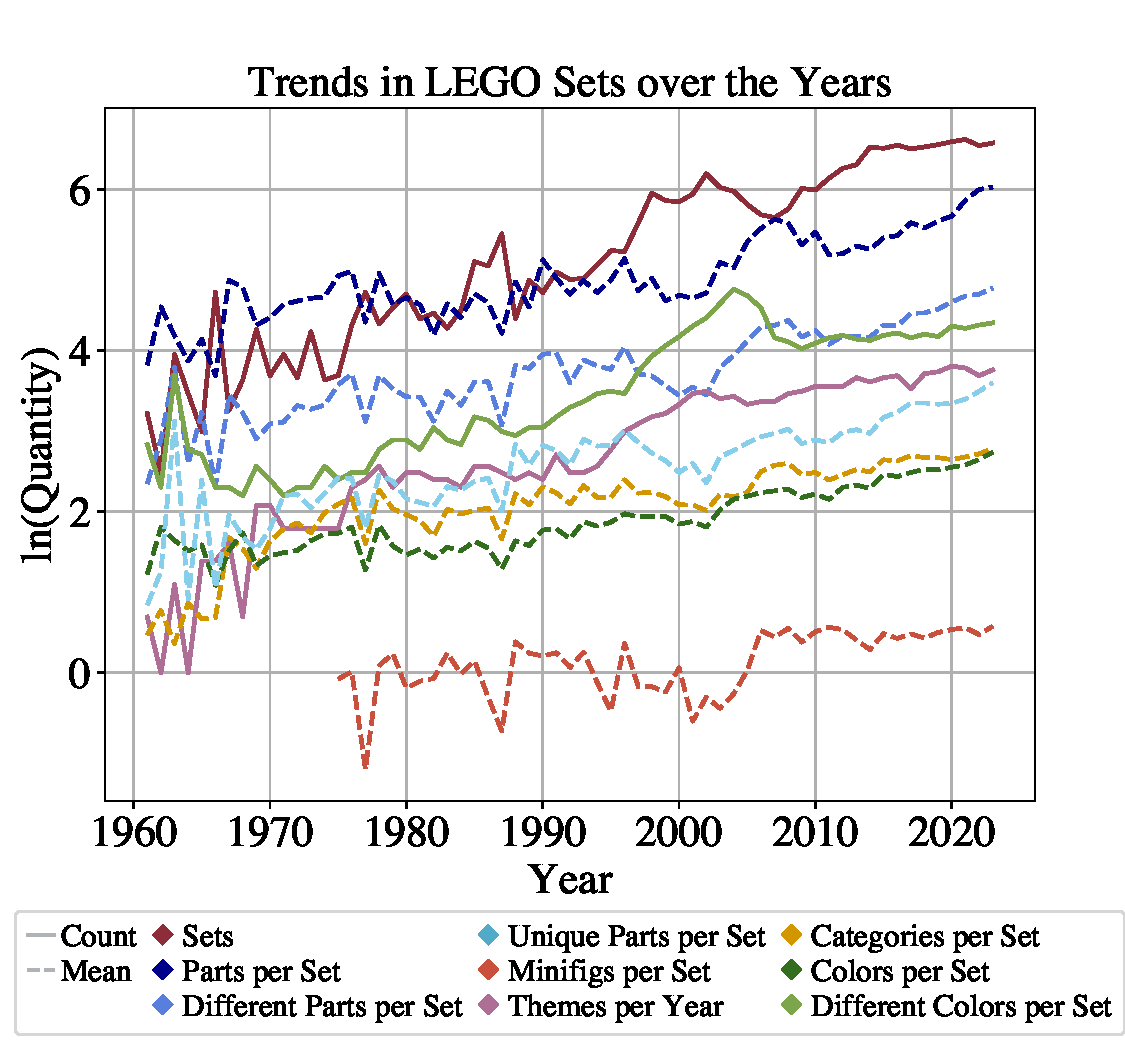
\includegraphics[width=\columnwidth]{../Images/Exploration.pdf}}
\caption{Trends of different features of LEGO sets over the years.}
\label{icml-historical}
 \end{center}
 \vskip -0.2in
\end{figure}
\vfill\eject,

Our exploration then involved analyzing the mean proportion of unique parts to non-unique parts per set per year. Additionally, the ten most used themes between 2000 and 2023 were identified using different criteria (number of sets, number of parts, most different parts) and we determined the ten most colors in those themes. Predictions for these metrics and the number of released sets and mean part count per set until 2030 were made using linear regression. These analyses can be found in the \href{https://github.com/eddiebeach99/Data_Literacy/blob/main/Analysis/exploratory_analysis.ipynb}{exploratory analysis file on github}. \\
We then introduced a metric to quantify the design complexity for each set, by linearly taking into account the variety of different features in each set to derive the following formula:
\[Comp = Parts + Diff + Cat + Uniq + Cols + Figs\]
where the features are defined as:
\begin{conditions*}
 Comp & Complexity\\
 Parts  &  Total number of parts\\
 Diff  &  Number of different parts \\
 Cat & Number of different categories of the parts\\
 Uniq  & Number of unique parts \\
 Cols & Number of different colors\\
 Figs & Number of minifigures\\
\end{conditions*}
The complexity metric was normalized to a range between 0 and 1, where a score of 1 represents the highest complexity and 0 the lowest. Normalization was achieved by applying the formula:
\[Complexity = \frac{Comp - MinComp}{MaxComp - MinComp}\]\\
where
\begin{conditions*}
 Complexity & Normalized complexity\\
 Comp & Complexity\\
 MinComp  &  Minimal complexity across all sets\\
 MaxComp  &  Maximal complexity across all sets \\
\end{conditions*}
Subsequently, we used regression analysis to identify any upward or downward trends in set complexity over the years. For this, a linear and exponential regression was employed to model the mean complexity per year, providing predictions until 2030. We visually compared the two regression lines and assessed their fit through the examination of the Sum of Squared Residuals ($SSR$) and Coefficient of Determination ($R^2$) to find the regression that better fits the data. We additionally checked the regressions for over- or underfitting using cross-validation, which is an efficient approach to identify such issues in regression models \cite{emmert2019evaluation}. \\
To analyze the different levels of complexity within LEGO sets and to see if the ratio of complex to simple sets has changed over the years, we performed a k-means cluster analysis. We used the same features as the complexity metric for cluster determination. The features were standardized to ensure equal contribution to the analysis. The elbow method was applied to determine the optimal number of clusters, which turned out to be three. We then computed the average number of features across sets within each complexity cluster and examined the relative distribution of sets in clusters across different years.

\section{Results}\label{sec:results}
The linear regression ($SSR = 0.002$, $R^2= 0.725$) and exponential regression ($SSR = 0.001$, $R^2= 0.805$) for the average complexity per set per year with a prediction until 2030 can be seen in Figure 2. The regression models suggest that the complexity rating has increased over the years. In the cross-validation of the two models we observed that both models show nearly the same mean of the Root Mean Square Error ($RMSE$) on the test set compared to the training set (linear regression: $RMSE_{training} = 0.005$, $RMSE_{test} = 0.005$; exponential regression: $RMSE_{training} = 0.004$, $RMSE_{test} = 0.003$). Further visualization, like the distribution of the complexity score, can be found in the \href{https://github.com/eddiebeach99/Data_Literacy/blob/main/Analysis/complexity_regression.ipynb}{regression file on github}.
\begin{figure}[H]
\vskip 0.2in
 \begin{center}
 \centerline{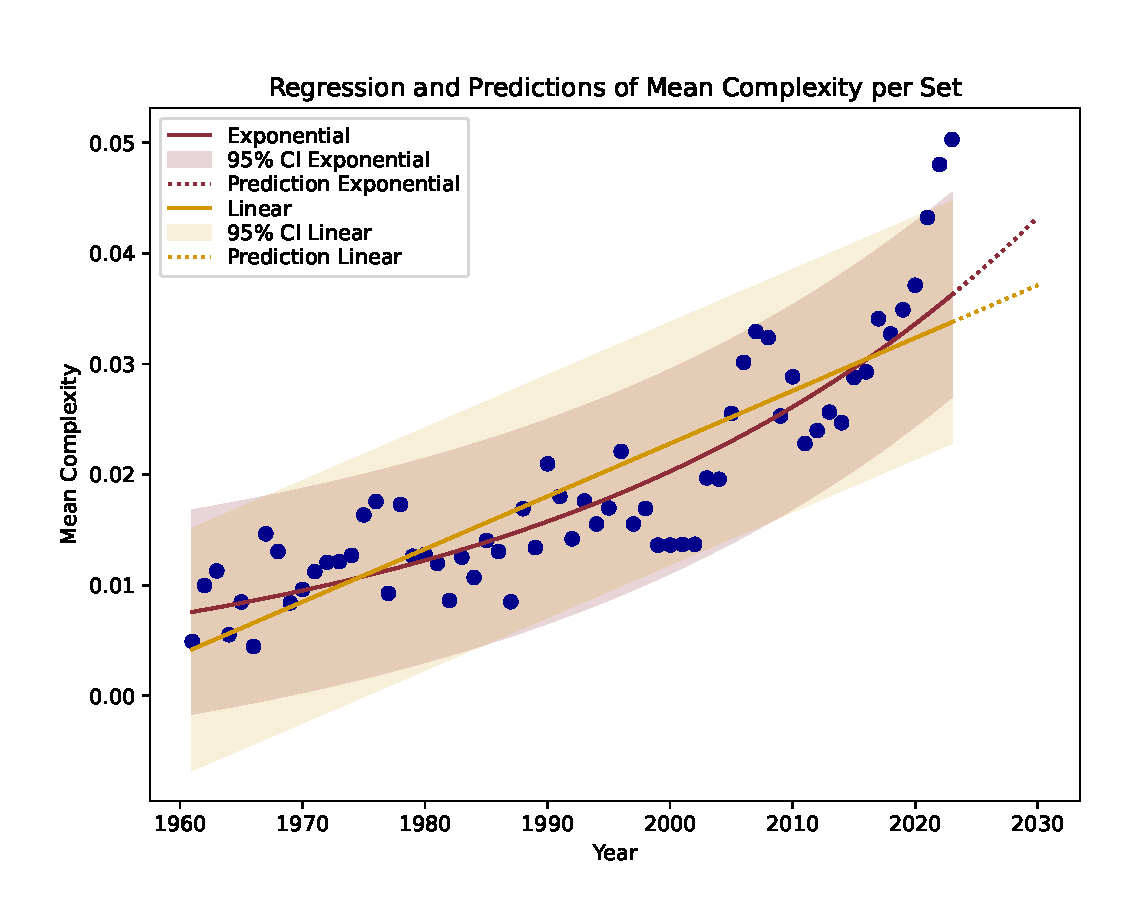
\includegraphics[width=\columnwidth]{../Images/Regressions.pdf}}
\caption{Exponential and linear regression of the mean complexity for a LEGO set per year with predictions until 2030.}
\label{icml-historical}
 \end{center}
\vskip -0.2in
\end{figure}
Results of the k-means clustering are presented in Figure 3, illustrating the mean values for each feature determining the cluster. The average complexity scores for the three clusters were 0.01, 0.06, and 0.23, respectively, with clusters ranked from low to high complexity based on their scores. Figure 3 indicates that the high complexity cluster contains larger average quantities in all features compared to the medium and low complexity clusters. Figure 4 depicts the relative percentage of sets in the different clusters over the years. Over time, there is an observable increase in the number of sets belonging to more complex clusters. Further visualization, like the top ten themes in the different complexity clusters, can be found in the \href{https://github.com/eddiebeach99/Data_Literacy/blob/main/Analysis/clustering.ipynb}{clustering file on github}.
\begin{figure}[H]
 \vskip 0.2in
 \begin{center}
 \centerline{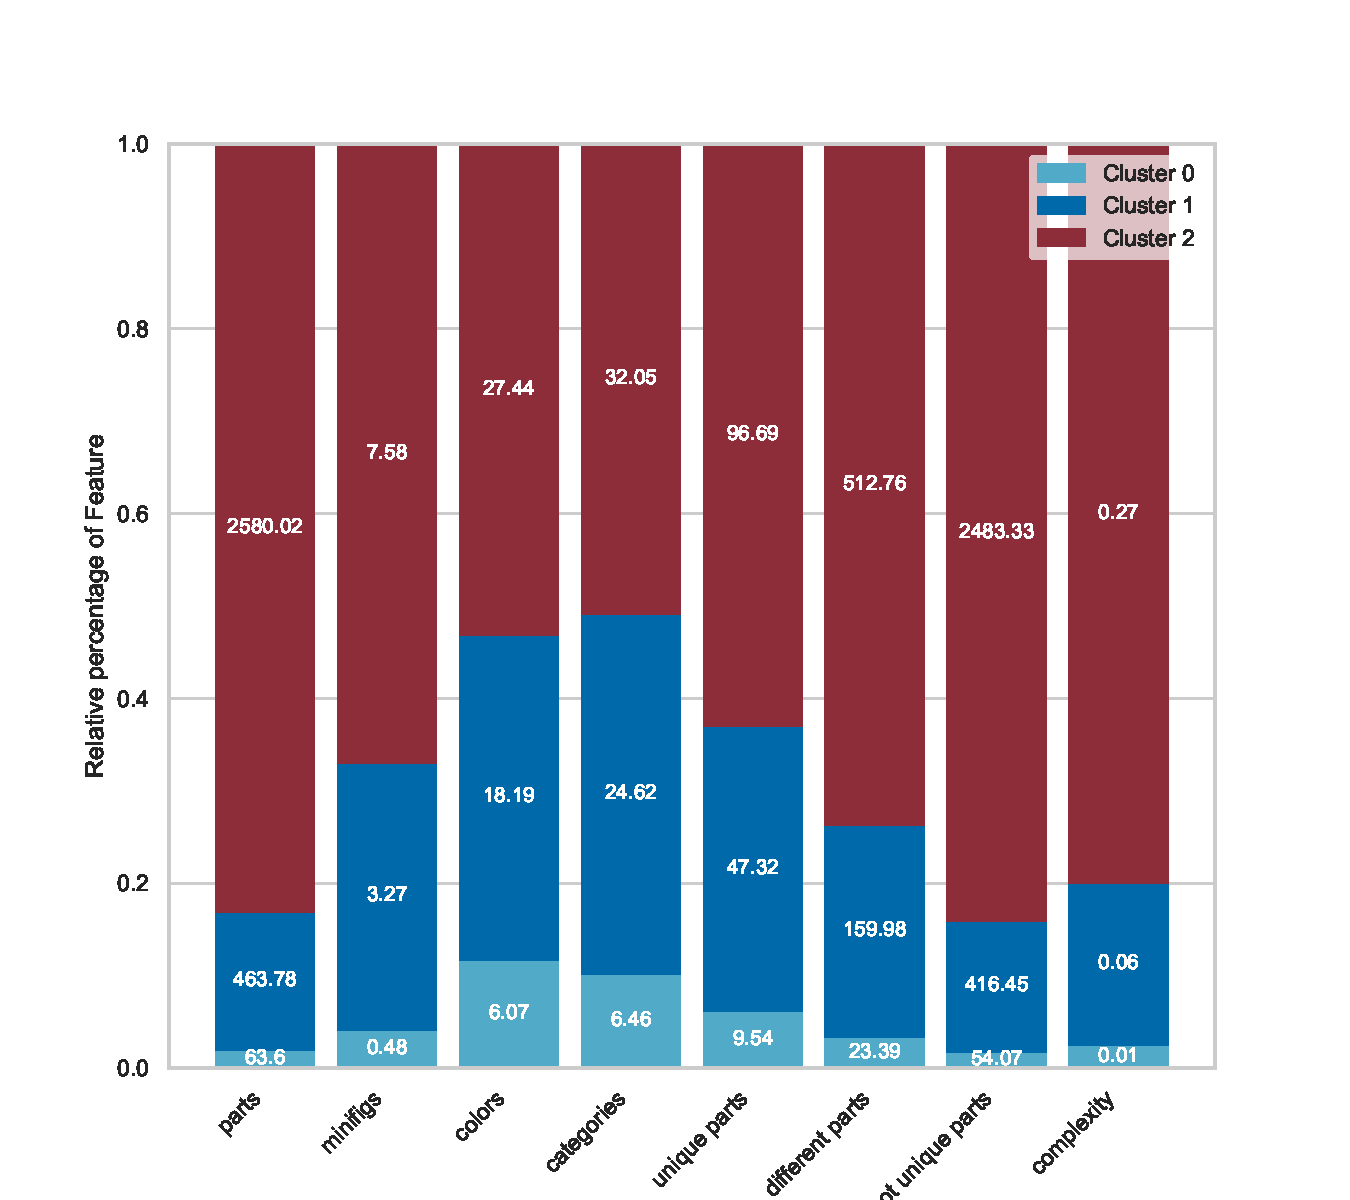
\includegraphics[width=\columnwidth]{../Images/Clusters_features.pdf}}
\caption{Proportion of features in the different clusters with values in the bar depicting the mean feature quantity.}
\label{icml-historical}
 \end{center}
 \vskip -0.2in
\end{figure}
\begin{figure}[H]
 \vskip 0.2in
 \begin{center}
 \centerline{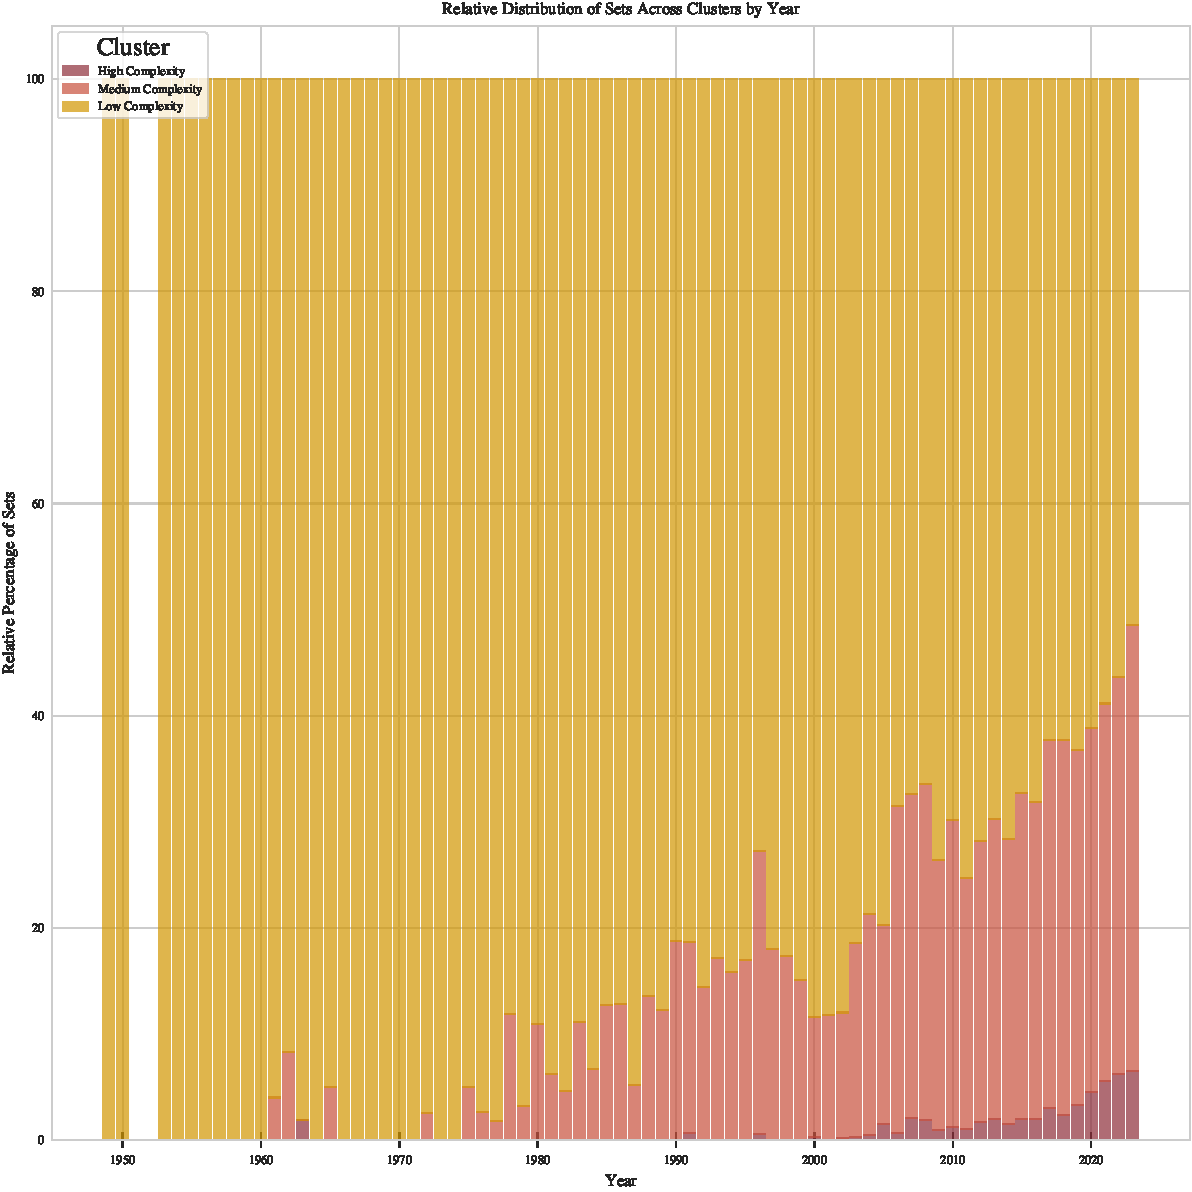
\includegraphics[width=\columnwidth]{../Images/Clusters.pdf}}
\caption{Proportion of sets in different clusters over the years.}
\label{icml-historical}
 \end{center}
 \vskip -0.2in
\end{figure}

\section{Discussion \& Conclusion}\label{sec:conclusion}

In this study, we performed an analysis of LEGO sets, exploring their design complexity over the years. Using the Rebrickable dataset from 1961 to 2024, we quantified complexity using factors such as part count, colors, and minifigures, among other factors. Our results, supported by regression and clustering analyses, showed a consistent upward trend in set design complexity. Linear and exponential regressions predicted sustained growth until 2030. Visual analysis of the regression models indicated that the exponential regression offers a more favorable fit to the data. This observation is underlined by a lower $SSR$ and a higher $R^2$ value compared to the linear regression. To further validate the models, we conducted cross-validation, revealing consistent performance on both training and unseen test data, suggesting no over- or underfitting. Notably, the exponential regression model displayed slightly lower $RMSE$ values, indicating a more accurate fit to the data. Thus, we assert that the complexity of LEGO sets has undergone exponential growth over the years. \\
Concurrently, k-means clustering identified three complexity clusters, showcasing an increasing proportion of sets in more complex categories over time. Interestingly, the optimal number of clusters determined through the k-means clustering analysis was three. This could suggest that LEGO intentionally categorizes its sets into distinct complexity levels, each catering to different target groups, where high complexity sets may be geared towards adults and low complexity sets geared toward younger children.\\
However, there are some limitations to consider. Given the limited number of set entries in the earlier years, there is a potential for these years to introduce a skew in the results when assessing the proportion of complex sets in each year. Additionally, various factors within the dataset show a correlation, such as the number of parts in a set and the likelihood of having many colors ($r=0.53$) or the number of parts and the number of different parts ($r=0.74$). This interdependence among factors could confound the true influence of each feature on set complexity. Furthermore, the absence of minifigures in LEGO sets until 1975 limits the assessment of complexity during those years, as this element became an important design component in later sets.
Nevertheless, we remain confident in the interpretability of our findings. While correlations exist among features, each factor independently contributes to the complexity of a LEGO set. For example, a set with a high number of parts may provide the potential for a greater variety of colors, but this doesn't necessarily imply more different colors have to be present. Moreover, considering the absence of minifigures in the very early years, our analysis suggests that this limitation has a relatively minor impact, as sets that feature minifigures starting from 1975 still demonstrate an increasing complexity rating over time. \\
We, therefore, conclude that the design complexity of LEGO sets experiences exponential growth, characterized by the release of increasingly complex sets in proportion to simpler ones.



\section*{Contribution Statement}

Patricia Schlegel prepared the data, calculated the complexity for each LEGO set, made first exploratory analyses and the two regressions of the complexity. Edward Beach performed the k-means clustering and revised the plots for the report. Both authors jointly wrote the text of the report.


\bibliography{bibliography}
\bibliographystyle{icml2023}

\end{document}

% This document was modified from the file originally made available by
% Pat Langley and Andrea Danyluk for ICML-2K. This version was created
% by Iain Murray in 2018, and modified by Alexandre Bouchard in
% 2019 and 2021 and by Csaba Szepesvari, Gang Niu and Sivan Sabato in 2022.
% Modified again in 2023 by Sivan Sabato and Jonathan Scarlett.
% Previous contributors include Dan Roy, Lise Getoor and Tobias
% Scheffer, which was slightly modified from the 2010 version by
% Thorsten Joachims & Johannes Fuernkranz, slightly modified from the
% 2009 version by Kiri Wagstaff and Sam Roweis's 2008 version, which is
% slightly modified from Prasad Tadepalli's 2007 version which is a
% lightly changed version of the previous year's version by Andrew
% Moore, which was in turn edited from those of Kristian Kersting and
% Codrina Lauth. Alex Smola contributed to the algorithmic style files.